\documentclass{article}

\usepackage[left=2.5cm,right=2.5cm,top=1.5cm,bottom=1.5cm]{geometry}

\usepackage[french]{babel}
\usepackage[utf8]{inputenc}
\usepackage[T1]{fontenc}

\usepackage{graphicx}
\graphicspath{{report/img/}}
\usepackage{subcaption}

\usepackage{amsmath, amssymb}
\usepackage{float}

\usepackage{hyperref}
\bibliographystyle{plainurl}

\usepackage[dvipsnames]{xcolor}

\usepackage{listings}
\usepackage{xcolor}  % Pour colorer si besoin

\lstdefinestyle{customc}{
  language=C,
  backgroundcolor=\color{gray!5},         % fond légèrement grisé
  frame=single,                           % encadrement
  rulecolor=\color{gray},                % couleur du cadre
  basicstyle=\ttfamily\footnotesize,     % police à chasse fixe
  keywordstyle=\color{blue}\bfseries,     % mots-clés en bleu gras
  stringstyle=\color{orange},            % chaînes en orange
  commentstyle=\color{gray!60}\itshape,  % commentaires gris en italique
  numbers=left,                          % numérotation à gauche
  numberstyle=\tiny\color{gray},         % style des numéros
  stepnumber=1,                          % numéro à chaque ligne
  tabsize=4,                             % taille des tabulations
  showstringspaces=false,               % ne pas afficher les espaces dans les chaînes
  breaklines=true,                      % retour à la ligne automatique
  morekeywords={vertex_t, gsl_spmatrix_uint},  % tes mots-clés ajoutés
}

%%%%%%%%%%%%%%%% Page de garde %%%%%%%%%%%%%%%%

\begin{document}

\begin{titlepage}
    \centering
    
\includegraphics[width=0.7\textwidth]{logo_em} \\
    \vspace{2cm}
    {\Huge \textbf{Rapport de projet S6}} \\
    \vspace{2cm}
    {\Large Lucie Pacou, Solan Boher-Sanchez, Tristan Collemiche, Yani Haouchine} \\
    \vspace{1cm}
    {\Large Enseirb-Matmeca} \\
    \vspace{1cm}
    {\Large Projet de programmation : Coursidor} \\
    \vspace{1cm}
    {\Large Encadrant : Trupin Loic}
    \vfill
    {\Large 2025} \\
\end{titlepage}

\tableofcontents
\newpage

%%%%%%%%%%%%%%%% Main part %%%%%%%%%%%%%%%%

\section{Introduction}

Les objectifs principaux de ce projet est d'implémenter la variante du jeu \textit{Quoridor} nommée \textit{Coursidor} avec des \textbf{clients} qui jouent à ce jeu et un \textbf{serveur} qui s'occupe de faire jouer des parties à deux \textbf{clients} à la fois sur différent \textbf{plateaux de jeu}, eux aussi à implémenter.
\bigskip

Ce projet est donc axé d'abord sur l'implémentation de jeu en C, l'utilisation de bibliothèque dynamique pour les \textbf{clients} et enfin surtout sur des problèmes d'algorithmiques de graphes pour l'implémentation des stratégies de jeu des \textbf{clients}.

\section{Structure du projet}

Cette section sera dédiée à l'explication et l'implémentation de nos structures de jeu ainsi que du principe de client/serveur.

\subsection{Structure de graphe et abstraction}

Le plateau de jeu \textit{Coursidor} est représenté par un graphe où chaque sommet correspond à une position possible d'un joueur et les arêtes correspondent aux déplacements possibles depuis les sommets.
Le graphe est plongé dans le plan c'est à dire que chaque sommet voit ses arêtes prendre 7 directions : \texttt{NO\_EDGE=0, NW=1, NE=2, E=3, SE=4, SW=5, et W=6}.
Il existe également une direction spéciale \texttt{WALL\_DIR} qui indique que la direction est bloquée par un mur.
Ces graphes sont implémentés en utilisant des matrices creuses de la \textit{GNU Scientific Library (GSL)}.
Il a donc été nécessaire de définir une abstraction en utilisant une interface pour utiliser ces matrices comme des graphes.

\begin{lstlisting}[style=customc, label={lst:graph}, caption={Définition du type graph\_t}]
  struct graph_t {
    enum graph_type_t type; // The type of the graph
    unsigned int num_vertices; // Number of vertices in the graph
    unsigned int num_edges; // Number of edges in the graph
    gsl_spmatrix_uint* t; // Sparse matrix of size num_vertices*num_vertices,
                          // t[i][j] > 0 means there is an edge from i to j
                          // t[i][j] == E means that j is EAST of i
                          // t[i][j] == W means that j is WEST of i
                          // and so on
    vertex_t start[NUM_PLAYERS]; // Starting vertices of both players
    unsigned int num_objectives; // Number of objectives in the graph
    vertex_t* objectives; // Objectives of the graph
};
\end{lstlisting}

Le listing \ref{lst:graph} nous renseigne sur les champs de notre structure \textit{graph\_t}.
Les valeurs dans la matrice du graphe aux indices \textit{i,j} correspondent à la direction de l'arête.

\begin{lstlisting}[style=customc, label={lst:graphprim}, caption={Primitives du type graph\_t}]
  struct graph_t* graph_create(unsigned int n_vertices);

  enum dir_t graph_exist_edge(struct graph_t* g, struct edge_t e);

  int graph_remove_edge(struct graph_t* g, struct edge_t e);

  int graph_add_edge(struct graph_t* g, vertex_t fr, vertex_t to, enum dir_t d);

  vertex_t graph_neighbor_direction(struct graph_t* g, vertex_t v, enum dir_t d);

  void graph_free(struct graph_t** g);

  void graph_dot(struct graph_t* g, struct edge_t* removed, int removed_size, vertex_t black_player_pos, vertex_t white_player_pos, char* name, int append);

  void graph_cpy(struct graph_t* dest, struct graph_t* src);

  unsigned int graph_get_num_vertices(struct graph_t* g);

  unsigned int graph_get_num_edges(struct graph_t* g);

  unsigned int graph_get_num_objectives(struct graph_t* g);
\end{lstlisting}

Les primitives données en listing \ref{lst:graphprim} ont donc été créées.
Ces fonctions permettent toutes les opérations nécessaires sur les graphes dans notre projet.
Ainsi, les matrices creuses \textit{GSL} n'apparaissent nulle part ailleurs que dans le fichier \textit{board.c} où sont implémentées ces fonctions.

\paragraph{Intérêts : }
Créer une interface de ce type permet une abstraction totale des matrices creuses et donc une totale modularité quant à leur implémentation.
Cela permet d'éviter les erreurs en rapport avec cette bibliothèque car celles-ci sont traitées dans les fonctions de l'interface.

\subsection{Mise en place des clients}

Pour tous les clients, l'interface client/serveur est la même. En effet, dans chaque fichier client \texttt{.c}, compilés par la suite sous la forme d'une bibliothèque partagée, est inclu le fichier d'en-tête \texttt{player.h}. Les quatre fonctions extraites des bibliothèques par le serveur et communes à tous les clients sont déclarées dans ce fichier.

Ces fonctions sont les suivantes :
\begin{lstlisting}[style=customc, label={lst:playerprim}, caption={Primitives du fichier player.h}]
 char const* get_player_name();

void initialize(unsigned int player_id, struct graph_t* graph);

struct move_t play(const struct move_t previous_move);

void finalize();
  \end{lstlisting}

L'intérêt de compiler les clients sous la forme de bibliothèques partagées est de pouvoir utiliser les clients après compilation du serveur et de les rendre ainsi intéropérables.

\subsection{Mise en place du serveur}

\subsubsection*{Utilisation des bibliothèques dynamiques}

Pour faire jouer deux clients ensemble, il faut charger leurs bibliothèques partagées dynamiquement.
Pour celà, on utilise des fonctions définies dans la bibliothèque \texttt{dlfcn.h}.
On utilise d'abord la fonction \texttt{dlopen} qui prend en paramètre le chemin vers la bibliothèque partagée et qui renvoit un pointeur \texttt{void*} qui représente une \textit{handle}, en français une poignée, sur la bibliothèque.

Pour accéder ensuite aux différentes fonctions du client, on utilise la fonction \texttt{dlsym} qui prend en paramètres deux arguments :
\begin{itemize}
\item un pointeur que l'on va faire pointer vers la fonction à laquelle on veut accéder
\item une chaîne de caractère qui est le nom de la fonction que l'on veut récupérer
\end{itemize}
Lorsque l'on utilise \texttt{dlopen} ou \texttt{dlsym}, il est préférable d'utiliser ensuite la fonction \texttt{dlerror}. Cette fonction renvoie un message d'erreur si l'accès à la bibliothèque ou à l'une des fonctions présentes dans celle-ci a rencontré un problème.

Enfin, pour fermer l'accès à la bibliothèque partagée, on utilise \texttt{dlclose} qui prend en argument la \texttt{handle} vers la bibliothèque (pointeur obtenu avec \texttt{dlopen}) et coupe ce lien.


\subsubsection*{Modularité}

Afin de rendre le code plus lisible, mais aussi d'augmenter son adaptabilité, nous avons rendu le code du serveur modulaire.
Nous avons ainsi défini une structure de données \texttt{player\_func}.
Elle contient les champs suivants :
\begin{itemize}
\item \texttt{void* player} : \texttt{handle} sur la bibliothèque partagée du client
\item \texttt{char* (*get\_player\_name)(void)} : pointeur vers la fonction \texttt{get\_player\_name} 
\item \texttt{void (*initialize)(unsigned int, struct graph\_t*)} : pointeur vers la fonction \texttt{initialize}
\item \texttt{struct move\_t (*play)(const struct move\_t)} : pointeur vers la fonction \texttt{play}
\item \texttt{void (*finalize)(void)} : pointeur vers la fonction \texttt{finalize}
\item \texttt{int num\_wins} : nombre de victoires du joueur
\item \texttt{struct graph\_t* graph\_player} : copie du graphe dans la structure du joueur
\item \texttt{vertex\_t initial\_position} : position initiale du joueur
\item \texttt{vertex\_t current\_position} : position actuelle du joueur
\item \texttt{int* objectives\_reached} : tableau de booléens indiquant si l'objectif a été atteint ou non
\item \texttt{enum dir\_t previous\_dir} : direction empruntée au dernier coup par le joueur
\item \texttt{int num\_wall} : nombre de murs placés
  \item \texttt{int lost} : booléen indiquant si le joueur a perdu ou non
\end{itemize}

\bigskip

Nous avons stocké les différentes structures \texttt{player\_func} décrivant les joueurs dans un tableau global \texttt{players} pour faciliter l'accès aux différents joueurs mais aussi dans un objectif de modularité.

\bigskip

Pour la suite de la mise en place du serveur, nous avons pensé le code de la manière la plus générale possible, nous avons donc fait en sorte qu'il soit adaptable à un contexte où une partie à plus de deux joueurs est possible.

Pour choisir aléatoirement lequel des joueurs sera le premier à jouer, nous avons tiré aléatoirement un nombre \texttt{i} entre 0 et \texttt{NUM\_PLAYER}, la macro définissant le nombre de joueur. Le premier joueur sera ainsi celui donc la bibliothèque partagée sera placée à l'indice \texttt{i} en ligne de commande (sans prendre en compte les options).
On charge ensuite les bibliothèques une par une dans leur ordre d'apparition après l'indice tiré dans le tableau \texttt{players}, avec le premier joueur à l'indice 0.

\subsubsection*{Boucle de jeu}

Le jeu est lancé dans la fonction \texttt{game}. L'intérêt de séparer la boucle de jeu du \texttt{main} est d'améliorer la lisibilité du code mais aussi de relancer plusieurs parties à la suite afin de tester le taux de réussite de la stratégie d'un client contre un autre.

Le graphe et d'autres paramètres sont initialisés selon les options données en ligne de commande : 
\begin{itemize}
\item \texttt{-t} : type de graphe (triangulaire, circulaire ou troué)
\item \texttt{-m} : taille de la maille
\item \texttt{-M} : nombre maximal de tours dans la boucle de jeu
  \item \texttt{-g} : nombre de boucles de jeu générées (utile pour tester la stratégie des clients)
\end{itemize}

Les joueurs sont ensuite initialisés par leur fonction propre \texttt{initialize} et ils jouent tour à tour avec leur fonction \texttt{play}.

La structure de donnée des coups \texttt{move\_t} est définie comme suit :
\begin{lstlisting}[style=customc, label={lst:move}, caption={Définition du type move\_t}]
  struct move_t {
    enum player_color_t c; // The color of the player
    enum move_type_t t; // The type of the move
    vertex_t m; // The id of a vertex
    struct edge_t e[2]; // The two edges for the wall
};

\end{lstlisting}

Lors d'un coup de type \texttt{MOVE}, le joueur peut accéder aux sommets suivants :
\begin{itemize}
\item sommets à une distance 1 et reliés par une arrête au sommet sur lequel est le joueur
\item sommets à un distance 2, ayant un angle de 30° avec la dernière direction empruntée par le joueur et étant reliés par des arêtes au sommet sur lequel est le joueur
  \item sommets à un distance 3, dans la même direction que la dernière direction empruntée par le joueur et étant reliés par des arêtes au sommet sur lequel est le joueur
\end{itemize}

\bigskip

La validité du coup retourné par la fonction \texttt{play} est ensuite vérifiée avec la fonction \texttt{is\_invalid}.
Cette fonction vérifie donc que le coup retourné ne commet pas les erreurs suivantes :
\begin{itemize}
\item le joueur joue un coup de type \texttt{MOVE} et veut rester sur sa position actuelle
  \item le joueur joue un coup de type \texttt{MOVE} et veut accéder à un sommet auxquel il ne peut pas accéder
\item le joueur joue un coup en essayant de se faire passer pour un autre joueur (la couleur de joueur indiquée dans son coup n'est pas la sienne)
\item le joueur joue un coup de type \texttt{WALL} et veut placer un mur qui rendra au moins un des objectifs inatteignables pour au moins un des joueurs
  \item le joueur joue un coup de type \texttt{WALL} mais il a déjà atteint son nombre maximal de murs posés
  \end{itemize}









\section{Stratégie client}

Dans cette section, nous allons nous intéresser à la partie stratégie des différents clients mis en place par notre équipe durant ce projet.

\subsection{Client naïf : Steven}

Pour pouvoir tester rapidement notre serveur avec un vrai joueur, nous avons commencé par coder un client naïf, affectueusement nommé \texttt{Steven}.
\bigskip

Ce joueur est codé pour toujours avancer d'un sommet vers l'Est. Si il ne peut pas, il reculera, donc avancera d'une case vers l'Ouest. Si il ne peut toujours pas, il choisira la première position disponible à une distance 1 en parcourant les directions dans le sens des aiguilles d'une montre. Si il ne trouve aucune position libre, c'est que le sommet sur lequel il se trouve est de degré 1 et que le joueur adverse est sur le sommet adjacent au sommet sur lequel est \texttt{Steven} puisque selon les règles du jeu, il ne peut être sur un sommet coupé de tout les autres. Dans ce cas là, il choisira de sauter au dessus de son adversaire.
\bigskip

Malgré sa simplicité, ce joueur nous a permi de bien cerner les règles du jeu et tester notre serveur en condition réelle. C'est pourquoi il est toujours intéressant de coder une stratégie naïve avant de s'intéresser à quelque chose de plus sofistiqué.

\subsection{Client basique : Tristan}

Quand nous avons ensuite voulu coder un joueur qui puisse pour de vrai jouer au jeu, nous nous sommes vite rendu compte que le client allait avoir besoin de toutes les informations de la partie, comme le serveur. Ce client est en fait doté d'un mini serveur qui s'occupe de récupérer les données transmises par le vrai serveur et de les utilisées pour actualiser son propre suivit de la partie qui se modélise par un plateau de jeu sous forme de graphe et des données relatives à chaque joueur présent dans la partie comme leur position, leur direction, les objectifs qu'ils ont ou non atteint, etc.
\bigskip

Une fois ceci mis en place, on peut s'occuper de l'établissement de la stratégie.

Pour notre joueur \texttt{Tristan}, la stratégie mise en place est la suivante. Quand le joueur souhaite décider d'un coup à jouer, il teste tout les coups valides qu'ils peut jouer et il donne à chaque coup une valeur définie par :
\[
valeur = (distance\_apres\_coup(\texttt{adversaire}) - distance\_apres\_coup(\texttt{Tristan}) -
\]
\[
(distance\_avant\_coup(\texttt{adversaire}) - distance\_avant\_coup(\texttt{Tristan}))
\]
Cela correspond à l'avance gagné par le joueur \texttt{Tristan} sur son adversaire grâce au coup joué.
\bigskip

Le graphe étant non pondéré, le plus court chemin est donné par un parcours en largeur. L'implémentation de ce parcours repose sur une structure de file (tableau circulaire). La distance est déterminée à partir de la position du joueur dont on cherche la distance à son objectif non visité le plus proche. Autrement dit, on part du principe qu'un joueur cherchera d'abord à atteindre l'objectif le plus proche de lui parmis ceux qu'il n'a pas encore atteint.

\begin{figure}[H]
\begin{minipage}[c]{.46\linewidth}
  \centering
  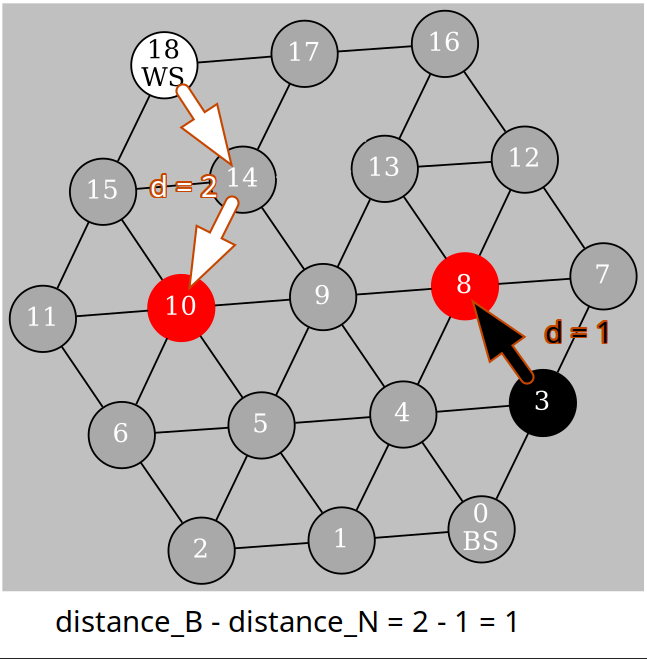
\includegraphics[width=\textwidth]{calcul_coup_avant.png}
  \caption{Distances avant le placement du coup}
  \label{fig:calcul_coup_avant}
\end{minipage}\hfill
\begin{minipage}[c]{.46\linewidth}
  \centering
  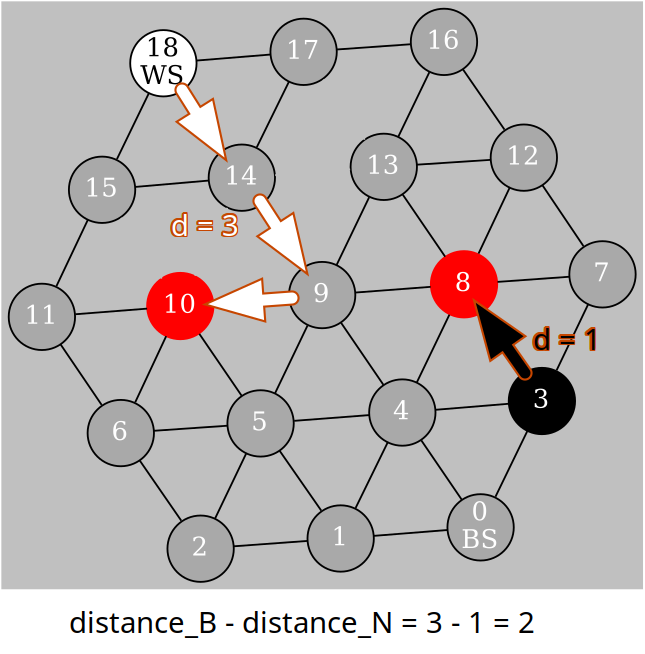
\includegraphics[width=\textwidth]{calcul_coup_apres.png}
  \caption{Distances après le placement du coup}
  \label{fig:calcul_coup_apres}
\end{minipage}
\end{figure}

Pour ce coup qui place un mur coupant les arêtes 15--10 et 14--10 entre les figures \ref{fig:calcul_coup_avant} et \ref{fig:calcul_coup_apres}, on obtient donc une valeur de 1:
\[
valeur = (3 - 1) - (2 - 1) = 2 - 1 = 1
\]
Ce coup a permi au joueur \texttt{Tristan} de gagner 1 d'avance sur son adversaire.
\bigskip

Une fois que chaque coup a été évalué, il est possible de déterminer la valeur donné la plus élevée. Le coup joué est désigné aléatoirement entre les coups ayant pour valeur cette valeur maximale.

\section{Construction des plateaux}

Bien que ne constituant pas une ``preuve'', la génération correcte du graphe est un ``argument'' convaincant en faveur du bon fonctionnement du programme.(Hypothèse H) 


\subsection{Plateau Triangulaire}
La construction du plateau triangulaire a été doublement importante. La première raison est que, étant le plus simple et le plus basique des 3 plateaux, son implémentation a servi de base à l'implémentation des 2 autres.

La deuxième raison est que, étant le premier plateau à avoir été codé et en raison de sa simplicité, c'est sur ce plateau que plusieurs tests seront faits, notamment les tests de stratégie. Pour ne pas avoir à discriminer sur la nature d'une erreur, il faut donc s'assurer que ce graphe a été construit de façon correcte.

\subsubsection*{Conception}

\paragraph{De bas en haut :} 
Le choix qui a été fait a été de construire le graphe de ``bas en haut'' en distinguant la ``phase de montée'' et la ``phase de descente''. Dans la ``phase de montée'', chaque ligne qui est au-dessus d'une autre possède un nœud de plus. Et dans la ``phase de descente'', chaque ligne au-dessus d'une autre contient un nœud de moins.     

\paragraph{Méthode du compteur :}
Chaque sommet étant représenté par un entier naturel durant la construction du graphe, on crée un compteur qui, à tout instant du programme, est égal au nombre représentant le sommet traité.

\subsubsection*{Implémentation}
De la conception précédente découle naturellement une implémentation constituée de deux boucles : la première correspondant à la ``phase montante'' et la deuxième correspondant à la ``phase descendante''. Chacune des deux boucles contient une boucle interne qui parcourt la ligne. La borne supérieure de cette boucle interne varie en accord avec la conception vue plus haut.

Dans la boucle interne, des disjonctions de cas sont faites selon l’emplacement du nœud dans la ligne.

\begin{lstlisting}[style=customc]
for (unsigned int i = 0; i < m - 1; i++) {
  for (unsigned int j = 0; j < m + i; j++) {
    // Phase montante 
  }
}
for (vertex_t i = m - 1; i > 0; i--) {
  for (vertex_t j = 0; j < m + i; j++) {
    // Phase descendante
  }
}
\end{lstlisting}

\paragraph{Remarque :}
Le nombre de sommets nous a été donné. Avec la méthode donnée plus haut, il aurait pu être calculé.

\subsubsection*{Terminaison}
Ce programme termine trivialement car il ne comporte pas de boucle while ni récursivité.

\subsubsection*{Correction}

Les figures \ref{fig:triangular3} et \ref{fig:triangular5} suffisent de preuve conformément à l'hypothèse H.

\begin{figure}[H]
\begin{minipage}[c]{.46\linewidth}
  \centering
  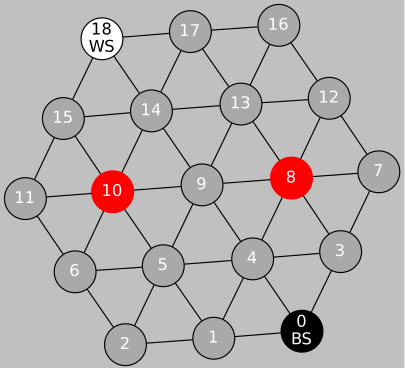
\includegraphics[width=\textwidth]{triangular3.png}
  \caption{Graphe triangulaire taille 3}
  \label{fig:triangular3}
\end{minipage}\hfill
\begin{minipage}[c]{.46\linewidth}
  \centering
  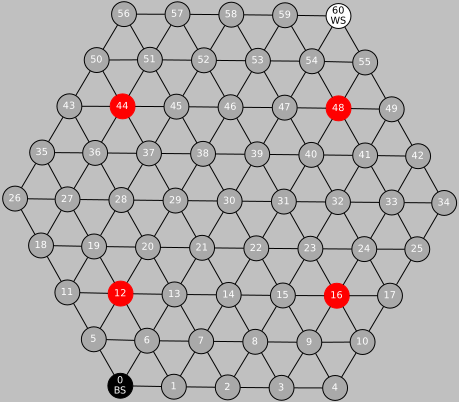
\includegraphics[width=\textwidth]{triangular5.png}
  \caption{Graphe triangulaire taille 5}
  \label{fig:triangular5}
\end{minipage}
\end{figure}

\subsubsection*{Complexité}

\paragraph{En temps :}
Soit $|S|$ le nombre de sommets du graphe, il y a exactement $|S|$ appels à la fonction \texttt{graph\_add\_edge} qui s'exécute en temps constant. La complexité est donc linéaire en la taille du graphe. Construire un graphe impliquant de construire l'ensemble de ses sommets, on peut légitimement penser que cette complexité est optimale.

\paragraph{En espace :}
Nous ne stockons que le graphe, aucun autre espace n'est alloué. La complexité spatiale est donc linéaire en la taille du graphe.

\subsection{Plateau circulaire}
Le plateau triangulaire a fait l'objet d'une mauvaise conception, ce qui a conduit à une mauvaise implémentation. Cette ``mauvaise'' implémentation, bien qu'inutile sur le plan pratique, fut vertueuse. Nous détaillons ce point plus bas.

\subsubsection*{Conception}
Similairement au plateau triangulaire, on retrouve la méthode du ``compteur'' et la construction de bas en haut décrites plus haut. Ici, les phases de montée et de descente sont indiscernables. Il y a néanmoins plus de disjonctions de cas que dans la construction du premier graphe :
\begin{itemize}
    \item Le premier cas correspond à la première ligne
    \item Le deuxième cas correspond à la deuxième ligne
    \item Le troisième cas correspond à la construction de la ``phase montante'' restante
    \item Le quatrième cas représente la construction de la ``phase descendante'' jusqu'à l'avant-avant-dernière ligne
    \item Le 5\textsuperscript{ème} cas correspond à l'avant-avant-dernière ligne
    \item Le 6\textsuperscript{ème} cas correspond à l'avant-dernière ligne
    \item Le dernier cas correspond naturellement à la dernière ligne
\end{itemize}

\subsubsection*{Implémentation}
De la conception découle 7 parties dans la fonction. Hormis la 5\textsuperscript{ème}, elles sont toutes représentées par des boucles.

\subsubsection*{Terminaison}
En l'absence de boucle \texttt{while}, ce programme termine trivialement.

\subsubsection*{Correction}

Les figures \ref{fig:circular3} et \ref{fig:circular5} suffisent de preuve conformément à l'hypothèse H.
\begin{figure}[H]
\begin{minipage}[c]{.46\linewidth}
  \centering
  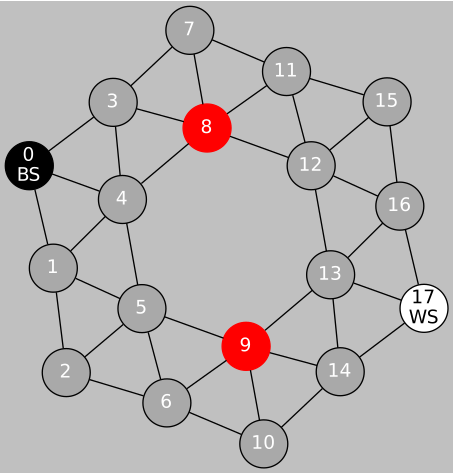
\includegraphics[width=\textwidth]{circular3.png}
  \caption{Graphe circulaire taille 3}
  \label{fig:circular3}
\end{minipage}\hfill
\begin{minipage}[c]{.46\linewidth}
  \centering
  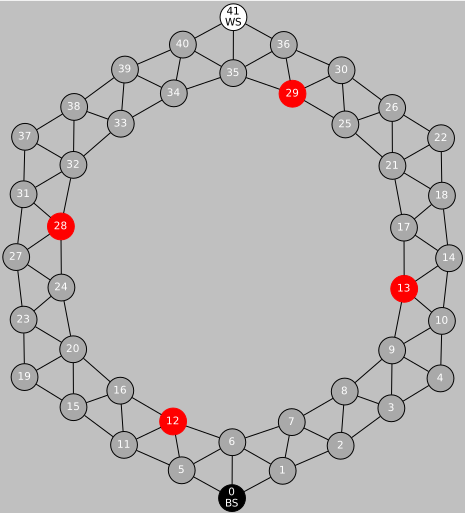
\includegraphics[width=\textwidth]{circular5.png}
  \caption{Graphe circulaire taille 5}
  \label{fig:circular5}
\end{minipage}
\end{figure}

\subsubsection*{Complexité}
\paragraph{Temporelle :}
La complexité de ce programme est linéaire en la taille du graphe, et pour les mêmes raisons exposées dans la partie graphe triangulaire, on admettra que la complexité est asymptotiquement optimale.

\paragraph{Spatiale :}
Linéaire en la taille du graphe.

\paragraph{Nota bene :}
Bien que la complexité soit optimale, on affirme ici que la conception de ce programme est mauvaise, pour plusieurs raisons :
\begin{itemize}
    \item Tout d'abord, il faut se remettre en contexte. Générer un graphe n'est pas une action qui sera répétée ; avoir une complexité suboptimale n'est donc pas tant gênant.
    \item Ensuite, tout comme le lecteur l'aura remarqué, la fonction \texttt{graph\_make\_circular} est compliquée. Elle n'utilise quasiment aucune sous-fonction. Le nombre de boucles, toutes avec des bornes différentes, augmente grandement le risque d'erreur. D'ailleurs, cette fonction fut la plus longue à coder parmi les trois.
    \item Enfin, plus une impression qu'un argument : une fois que le programme fut opérationnel, le code n'était toujours pas maîtrisé par ses développeurs. Il fonctionnait, mais beaucoup de choix ont été mis en place ``pour que ça marche'' et non apportés par une réelle compréhension.
\end{itemize}

Toutes ces erreurs furent bénéfiques pour les jeunes programmeurs que nous sommes pour la simple et bonne raison qu'elles sont venues souligner l'intérêt de ne pas passer trop vite à l'implémentation, et aussi et surtout de développer des ``outils'' fiables pour résoudre un problème.

\subsection{Plateau troué}
De par sa structure plus complexe et les erreurs faites durant la construction du graphe circulaire, la conception du graphe troué fut précédée par la conception d'outils aidant à la programmation.

\subsubsection*{Conception}
L'idée principale pour construire ce graphe sera de partir du graphe triangulaire, filtrer certains sommets de façon à obtenir le graphe troué.

La première idée est de faciliter le déplacement dans le graphe triangulaire. Pour cela, on veut une fonction qui prend en entrée une ligne $i$ et une colonne $j$ et qui renvoie le numéro du sommet se trouvant à l'intersection de la ligne $i$ et la colonne $j$.

Il faut à présent pouvoir ``représenter'' les trous, les distinguer, les définir.
Nous avons choisi pour cela de repérer leurs centres se situant à des positions constantes en fonction de $m$.

Une fois muni de ces représentants, savoir si un sommet existe ou non dans le graphe troué devient une tâche simple. Soit $v$ un sommet et soit $R$ le rayon d'un trou, s'il existe un représentant $r_i$ tel que $\|v - r_i\| < R$, alors $v$ n'existe pas dans le graphe troué, avec $\|\cdot\|$ la distance induite par le parcours du graphe.

Il s'agit à présent de pouvoir ``superposer'' le graphe troué et le graphe triangulaire.
Pour cela, on construit un mapping qui, à un sommet $i$ dans le graphe triangulaire, associe son numéro dans le graphe troué, $-1$ sinon. Ainsi, si $\text{map}(i) \neq -1$ et $\text{map}(j) \neq -1$ et si $j$ et $i$ sont reliés dans le graphe triangulaire, alors $\text{map}(i)$ et $\text{map}(j)$ sont reliés dans le graphe troué.

\subsubsection*{Implémentation}

\paragraph{Repérage}
On repère d'abord la position du premier élément de chaque ligne avec la fonction \texttt{first\_of\_ligne}. On distingue les cas où nous nous trouvons dans la partie haute ou basse du graphe pour profiter des symétries. Une fois avoir trouvé le premier élément de la $i$-ème ligne, il suffit de rajouter $j$ pour se retrouver à l'intersection de la $i$-ème ligne et de la $j$-ème colonne.

\begin{lstlisting}[style=customc]
vertex_t idx_2(size_t ligne, size_t colonne, size_t m) {
  return (vertex_t)(colonne + first_of_ligne(ligne, m));
}
\end{lstlisting}

\paragraph{Représentant}
À l'aide d'une feuille et d'un crayon, on trouve les coordonnées des représentants. Il suffit ensuite de les stocker dans un tableau.

\begin{lstlisting}[style=customc]
   representant[0] = idx_2(m - 1, m - 1, m);
   representant[1] = idx_2(m - 1, m + (m / 3) - 1 + (m / 3) - 1, m);
   ...
\end{lstlisting}

\paragraph{Filtre}
Muni de la fonction \texttt{bfs}, on obtient la distance entre deux points. On itère sur le tableau obtenu plus haut dans la fonction \texttt{exist} pour savoir, conformément à ce qui a été dit plus haut, si un sommet appartient au graphe troué.

\begin{lstlisting}[style=customc]
  int exist_graph_vertices(size_t m, vertex_t v, struct graph_t* g, vertex_t* representant) {
    for (int i = 0; i < 7; i++) {
      if ((In(representant[i], (m / 3 - 1), g, v))) {
        return 0;
      }
    }
  }
    return 1;
  \end{lstlisting}
  \begin{lstlisting}[style=customc]
  int In(vertex_t center, size_t radius, struct graph_t* g, vertex_t point) {
    if (bfs(g, center, point) < (int)radius)
        return 1;
    return 0;
}
\end{lstlisting}

\paragraph{Mapping}
On itère sur un tableau \texttt{map} pour associer le numéro de $i$ dans le graphe triangulaire au numéro de $i$ dans le graphe troué, $-1$ sinon. On procède ensuite comme décrit plus haut.

\begin{lstlisting}[style=customc]
  for (vertex_t i = 0; i < triang->num_vertices; i++) {
    map[i] = exist[i] ? num_vertices++ : (vertex_t)-1;
  }
\end{lstlisting}

\subsubsection*{Terminaison}
En l'absence de boucle \texttt{while}, nos fonctions terminent.

\subsubsection*{Correction}

Les figures \ref{fig:holey6} et \ref{fig:holey9} suffisent de preuve conformément à l'hypothèse H.
\begin{figure}[H]
\begin{minipage}[c]{.46\linewidth}
  \centering
  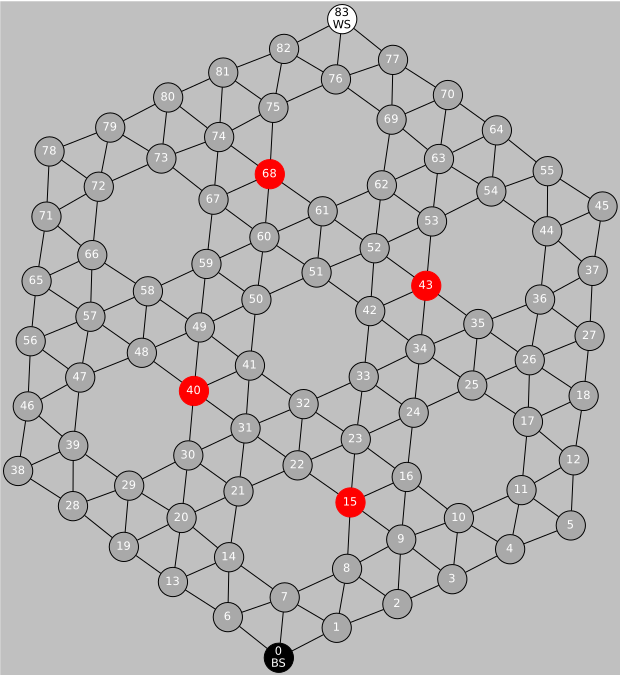
\includegraphics[width=\textwidth]{holey6.png}
  \caption{Graphe troué taille 6}
  \label{fig:holey6}
\end{minipage}\hfill
\begin{minipage}[c]{.46\linewidth}
  \centering
  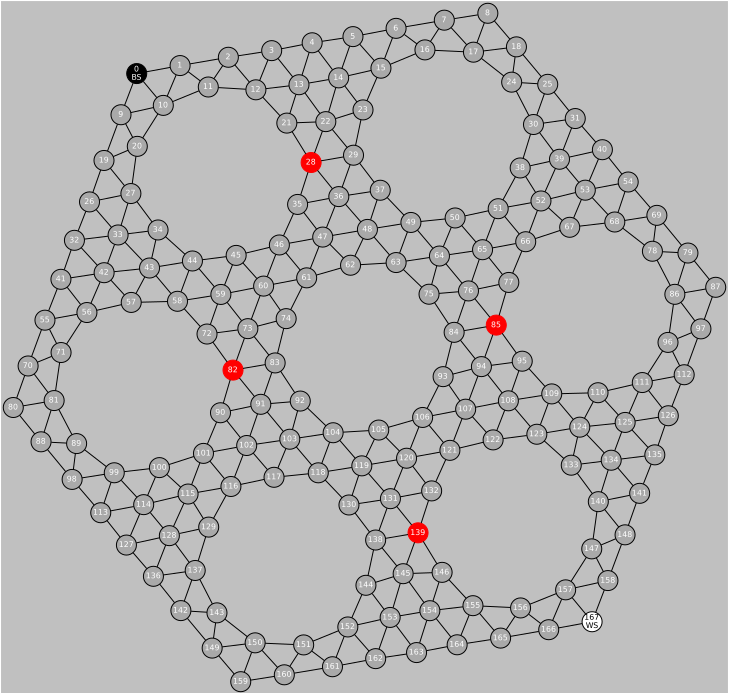
\includegraphics[width=\textwidth]{holey9.png}
  \caption{Graphe troué taille 9}
  \label{fig:holey9}
\end{minipage}
\end{figure}

\subsubsection*{Complexité}
La complexité provient majoritairement de la boucle construisant le mapping. Il y a $n$ itérations avec, pour chaque itération, un appel à \texttt{existe} qui appelle \texttt{In} qui appelle \texttt{bfs}, dont la complexité est classiquement linéaire en la taille du graphe. La complexité est donc quadratique en la taille du graphe.

La complexité est suboptimale.

\subsubsection*{Remarque}
\begin{itemize}
    \item Les symétries inhérentes aux graphes n'ont peut-être pas assez été utilisées.
    \item La complexité des fonctions de fin \texttt{gsl\_spmatrix\_uint(i)} n'a pas été prise en compte.
    \item Les techniques utilisées pour créer le graphe troué sont particulièrement utiles car elles permettraient de créer d'autres graphes de façon simple. Par exemple, en remplaçant les représentants par un unique représentant, on pourrait créer un graphe troué uniquement au centre dont le rayon du trou peut être choisi. En particulier, pour $r = m - 2$, on obtient le graphe circulaire. Il faut bien sûr penser à compter le nombre de sommets que contient chaque graphe pour pouvoir effectuer le \texttt{malloc}.
    \item La remarque ci-dessus pourrait mener à la conception d'une fonction générique pour générer les graphes... \#RENAULT
    \item Les complexités sont calculées en fonction de la taille du graphe et non en fonction de la taille de l'entrée. Si c'était le cas, l'entrée étant un entier $m$, les complexités en temps et en espace seraient exponentielles.
\end{itemize}



\section{Difficultés rencontrées}
Cette section a pour objectif de traiter toutes sortes de difficultés que nous avons rencontrés au cours du projet.

\subsection{Matrice CSR et COO}
Dans le cadre de l'abstraction des matrices pour notre type \texttt{graph\_t} il nous a été nécessaire d'utiliser les fonctions de \textit{GSL} pour les matrices creuses.

Il existe plusieurs implémentation des matrices creuses dans la library \textit{GSL}, dans notre cas l'implémentation \textit{CSR}, que l'on ne va expliciter ici, est celle choisi.
Cependant, les matrices \textit{CSR} ne permettent pas d'ajouter d'élément, il est nécessaire d'ajouter des éléments dans une matrice \textit{COO}, une autre implémentation, puis de la transformer en \textit{CSR}.
C'est particulièrement nécessaire dans le cas de la génération des graphes abordées précédemment, celle-ci est réalisé sur des matrices \textit{COO}.
\bigskip

Nous n'avions pas remarqué ça au départ et il a ainsi fallu adapter les primitives de notre type \texttt{graph\_t} pour changer leurs comportement selon le type de la matrice.
Par exemple, notre fonction \texttt{graph\_add\_edge} doit différencier les 2 types de matrices.
Dans le cas \textit{COO} elle utilise la fonction \texttt{set} de \textit{GSL} pour affecter une valeur à une position dans la matrice et dans l'autre cas la fonction \texttt{ptr} qui récupére le pointeur vers la valeur dans la matrice (pointeur qui ne peux exister si la valeur n'existe pas).

\subsection{Deboggage d'erreurs sur du code utilisant l'aléatoire}

Lors des tests de la fonction \texttt{play()} de \texttt{Tristan}, certaines erreurs sont évidemment advenues, notamment des erreurs faisant jouer certains coups interdits. Pour trouver les raisons qui faisaient jouer ces coups normalement impossibles à jouer, il paraissait naturel d'utiliser l'outil \texttt{gdb}.

Malheureusement, la décision du prochain coup du client \texttt{Tristan} étant aléatoire, il était impossible quand une erreur était remarquée de relancer la même partie avec \texttt{gdb} pour corriger précisément cette erreur. Et il était impossible de lancer une partie avec \texttt{gdb} en espérant réobtenir l'erreur. Certaines sont rares et cela aurait été beaucoup trop long.

La solution trouvée était de modifier temporairement l'implémentation de la fonction \texttt{play()} (dans le client et dans \texttt{player.h}) pour mettre en entrée de la fonction un argument \texttt{int seed}, qui permet de choisir sur quel aléatoire les coups du client seront choisis. Dans le même temps, on lance l'aléatoire avec la fonction \texttt{time(NULL)} dans le serveur, on affiche la valeur de time(NULL) et on la donne à la fonction \texttt{play()}.

Finalement, il ne restait plus qu'à lancer des parties en cherchant l'erreur avec l'affichage des parties - ce qui est donc rapide - et on relance la partie avec la \texttt{seed} - qui a été affiché par le serveur - en utilisant \texttt{gdb}.

\section{Tests de validation}
Il est important de pouvoir tester son code et nous l'expliquons succintement dans cette partie.

\subsection{Tests structurels}

Plusieurs test ont été réalisés sur les clients pour vérifier le bon respect des règles du jeu.%huyjtfrgklggujh(Camille)
D'autres tests succints ont été réalisés sur certaines fonctions.

La meilleure façon de valider le fonctionnement de nos clients reste de les faire s'affronter et d'observer le graphe de jeu obtenu dont nous discutons dans la prochaine partie.

\subsection{Affichage des parties}

Un autre moyen de tester le bon fonctionnement de nos clients ou du serveur est simplement d'observer le graphe du jeu.
Dans ce sens il nous a été nécessaire de créer une fonctions d'affichage des graphes avec les joueurs.

C'est ainsi que l'on a utilisé \textit{DOT}, un language de description de graphe.
Ce language nous permet de générer un graphe pour chaque état de la partie, le tout dans un pdf.
C'est le but de la fonction \textit{graph\_dot} qui a été apercu précédemment mais non expliqué.
Celle-ci génére un fichier \textit{DOT} qui est un simple fichier texte décrivant le graphe, ce fichier est ensuite compilé en pdf en utilisant \textit{neato}.
Il nous a également fallu créer un script bash pour lier chaque pdf de chaque graphe.
Ainsi, on obtient un pdf du nombre de page correspondant au nombre de coup de la partie.

\begin{figure}[H]
  \centering
  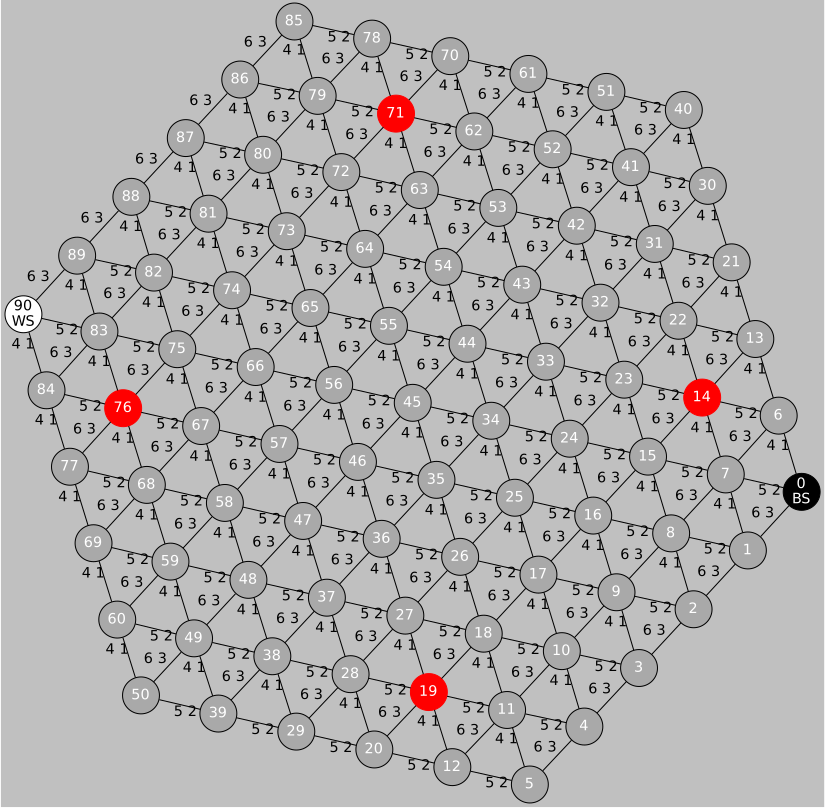
\includegraphics[width=0.8\textwidth]{dot.png}
  \caption{Affichage du plateau de jeu}
  \label{fig:dot}
\end{figure}


La figure \ref{fig:dot} montre un début de partie avec 4 objectifs, le joueur noir sur le sommet 0 et le joueur blanc sur le sommet 90. 

\section{Conclusion}

Ce projet fut vaste, à la fois sur les plans du développement logiciel, de l’algorithmie et de la théorie. Nous avons appris à gérer des serveurs, à créer des bibliothèques dynamiques.
Nous avons aussi appris à prendre du recul sur un problème afin de créer des outils nous permettant de résoudre ces mêmes problèmes.
Enfin, nous avons dû concevoir une stratégie, la tester, la comparer à d'autres, la remettre en question, puis la peaufiner.
En résumé, le projet Coursidor fut enrichissant à bien des égards pour les jeunes programmeurs que nous sommes.



\end{document}
